\documentclass[12pt,oneside]{report}

\usepackage[utf8]{inputenc}
\usepackage{biblatex}
\addbibresource{./reference.bib}
% linktocpage shall be added to snippets.

% \usepackage{hyperref,theoremref}
% \hypersetup{
% 	colorlinks, 
% 	linkcolor={red!40!black}, 
% 	citecolor={blue!50!black},
% 	urlcolor={blue!80!black},
% 	linktocpage % Link table of content to the page instead of the title
% }

\usepackage{subfiles}
\usepackage{blindtext}
\usepackage{tikz}
\usepackage{tikz-cd}
\usepackage{tcolorbox}
\tcbuselibrary{breakable}

\usetikzlibrary{cd}
\usetikzlibrary{positioning}

\usepackage{amssymb}
\usepackage{mathtools}
\usepackage{titlesec}
\usepackage{amsthm}
\usepackage{thmtools}
\usepackage{amsmath}
\usepackage{amssymb}
\usepackage{graphicx}
\usepackage{titlesec}
\usepackage{xcolor}
\usepackage{multicol}
% \usepackage{hyperref}
\usepackage{import}
\usepackage{algorithm}
\usepackage{algpseudocode}
\usepackage[toc,page]{appendix}
\usepackage{listings}
\lstdefinestyle{cppstyle}{
    language=C++,
    basicstyle=\ttfamily\footnotesize,        % Small but readable font
    keywordstyle=\color{blue}\bfseries,       % Keywords in blue and bold
    stringstyle=\color{teal},                 % Strings in teal
    commentstyle=\color{gray}\itshape,        % Comments in italic gray
    morecomment=[l][\color{magenta}]{\#},     % Preprocessor directives in magenta
    numbers=left,                             % Line numbers on the left
    numberstyle=\tiny\color{gray},            % Small gray line numbers
    stepnumber=0,                             % Number every line
    frame=single,                             % Add a thin border around the code
    rulecolor=\color{black},                  % Border color
    tabsize=4,                                % Set tab width
    breaklines=true,                          % Enable line wrapping
    breakatwhitespace=true,                   % Break at spaces
    showspaces=false,                         % Hide space markers
    showstringspaces=false,                   % Hide spaces in strings
    captionpos=b,                             % Caption at bottom
    aboveskip=5pt,                            % Space before code block
    belowskip=5pt,                            % Space after code block
    backgroundcolor=\color{black!5},          % Light gray background
}

\lstdefinestyle{python}{
    language=Python,
    basicstyle=\ttfamily\footnotesize,        
    backgroundcolor=\color{black!5},    % Light gray background
    keywordstyle=\bfseries\color{blue}, % Bold blue keywords
    stringstyle=\color{teal},           % Teal strings
    commentstyle=\color{gray},          % Gray comments
    stepnumber=0,                             % Number every line
    frame=single,                             % Add a thin border around the code
    rulecolor=\color{black},                  % Border color
    tabsize=4,                                % Set tab width
    breaklines=true,                          % Enable line wrapping
    breakatwhitespace=true,                   % Break at spaces
    showspaces=false,                         % Hide space markers
    showstringspaces=false,                   % Hide spaces in strings
    captionpos=b,                             % Caption at bottom
    aboveskip=5pt,                            % Space before code block
    belowskip=5pt,                            % Space after code block
    backgroundcolor=\color{black!5},          % Light gray background
}


\newtheorem{thm}{Theorema}[chapter]
\newtheorem{lemma}[thm]{Lemma}
\newtheorem{coro}[thm]{Corollarium}
\newtheorem{prop}[thm]{Propositio}
\theoremstyle{definition}
\newtheorem{defn}[thm]{Definitio}

\theoremstyle{definition}
\newtheorem{axiom}[thm]{Axioma}
\newtheorem{observation}[thm]{Observation}

\theoremstyle{remark}
\newtheorem{remark}[thm]{Observatio}
\newtheorem{hypothesis}[thm]{Coniectura}
\newtheorem{example}[thm]{Exampli Gratia}

\renewcommand\emptyset{\varnothing}
\renewcommand\mod{\text{ mod }}
%TODO mayby proof environment shall have more margin
% \renewenvironment{proof}{\vspace{0.4cm}\noindent\small{\emph{Demonstratio.}}}{\qed\vspace{0.4cm}}
% \renewenvironment{proof}{{\bfseries\emph{Demonstratio.}}}{\qed}
\renewcommand\qedsymbol{Q.E.D.}
% \renewcommand{\chaptername}{Caput}
% \renewcommand{\contentsname}{Index Capitum} % Index Capitum 
\renewcommand{\emph}[1]{\textbf{\textit{#1}}}
\renewcommand{\ker}[1]{\operatorname{Ker}{#1}}

%\DeclareMathOperator{\ker}{Ker}

% New Commands
\newcommand{\bb}[1]{\mathbb{#1}} %TODO add this line to nvim snippets
\newcommand{\orb}[2]{\text{Orb}_{#1}({#2})}
\newcommand{\stab}[2]{\text{Stab}_{#1}({#2})}
\newcommand{\im}[1]{\text{im}{\ #1}}
\newcommand{\se}[2]{\text{send}_{#1}({#2})}
\newcommand{\be}{b_\text{eff}}
% \renewcommand{\L}{L_{\lambda}(x)}

% project specific macros
% m stands for maximum
\newcommand{\mx}{\overline{x}}


\usetikzlibrary{arrows,calc,shadows.blur}
\tcbuselibrary{skins}
\newtcolorbox{nb}[1][]{%
	enhanced jigsaw,
	colback=gray!20!white,%
	colframe=gray!80!black,
	size=small,
	boxrule=1pt,
	title=\textbf{N.B.},
	halign title=flush center,
	coltitle=black,
	breakable,
	attach boxed title to top left={xshift=1cm,yshift=-\tcboxedtitleheight/2,yshifttext=-\tcboxedtitleheight/2},
	minipage boxed title=1.5cm,
	boxed title style={%
			colback=white,
			size=fbox,
			boxrule=1pt,
			boxsep=2pt,
			underlay={%
					\coordinate (dotA) at ($(interior.west) + (-0.5pt,0)$);
					\coordinate (dotB) at ($(interior.east) + (0.5pt,0)$);
					\begin{scope}
						\clip (interior.north west) rectangle ([xshift=3ex]interior.east);
						\filldraw [white, blur shadow={shadow opacity=60, shadow yshift=-.75ex}, rounded corners=2pt] (interior.north west) rectangle (interior.south east);
					\end{scope}
					\begin{scope}[gray!80!black]
						\fill (dotA) circle (2pt);
						\fill (dotB) circle (2pt);
					\end{scope}
				},
		},
	#1,
}

\date{27 February, 2025}
\title{Quantifying Chaos}
\author{Luc Dixon, Yuhao Han, Logan Hinkley}

\usepackage[y4project,fancyhdr,hyperref,colour]{edmaths}
\renewcommand{\L}{L_{\lambda}}
\flushbottom


\begin{document}
% \pagenumbering{roman}
\maketitle
\begin{abstract}
Chaos is an universal phenomenon observed in every aspect of the physical world. Examples include weather systems, celestial movements, demographic evolutions, and economic activities. 
The descriptions thereof often comprise of the adjective ``unpredictable,'' ``disordered'', ``entropic,'' ``confusing'', subject on to chances, and, in summary, ``chaotic''.
It may be of surprise that much more can be said to the even the simplest example.
In this report, however, we will demonstrate there are rich, universal, and quantitative mathematic properties shared by all of these chaotic systems.

We begin by introducing examples of chaos and their defining characteristics. 
The intuitive descriptions of chaos, as will be shown, can be rigorously described by Liapunov exponents and fractal dimensions.
After this, the iterative logistic map as a model of population is studied in details, which exhibit an interesting behavior of periodic bifurcations to chaos that is also observed among a large class of dynamical systems. 
The pinnacle of this report, presented in the last chapter, after developing some mathematically rigorous tools to study chaos, is the demonstrations of Feigenbaum's universal constants of bifurcation.
\end{abstract}

\declaration
\dedication{Musa mihi causas memora ...\\
	Muse, tell me the cause...
}

\tableofcontents

\chapter{Bifurcations in Discrete Dynamical Systems}
\section{The Logistic Map as Model for Population Growth}

One dimensional recursive equations $x_{n+1} = f(x_n)$ are used for modeling various dynamical systems. 
Its simplicity makes it easy to study, and many of its properties are also inherited by their more complicated counterparts.

Consider, for example, bacteria population in discrete time intervals. 
If the population is low and resource abundant, the rate of growth is in porportion to the population, which give rise to the following equation

$$
p_{t+1} = p_{t} b,
$$
where $p_{t}$ is the population of the bacteria at the dicrete time $t$ and $b$ as a constant is the static birth rate for bacteria whose value will depend on the model.

The limited resource will slow down the rate of growth as the population increases, and the the relation will become 

$$
	p_{t+1} =  p_{t} \be
$$

The usual assumption is that $\be$ is close to $b$ when the population is low, and there is a threshold which the population will never surpass. At the threshold $\be$ will be zero.

The simplest equation for modelling $\be$ is the linear equation

$$
\be = b - ap,
$$

where $a$ is another constant.
Combining the two, the recursive formula becomes 

$$
p_{t+1}  = b p_t - ap_t^2
$$

Substituting $p_{t} := \frac{b}{a} x_{t}, \lambda := \frac{b}{4}$, we obtain

$$
x_{t+1} = 4 \lambda x_t(1-x_t) 
$$

Indeed, thence come the standard forms of the logistic map

\begin{equation}\label{eq_logistic}
	L_{\lambda}(x) = 4 \lambda x(1-x)
\end{equation}

% graph produced by `logistic_map_diff_lambda`
\begin{figure}[t]
	\centering
	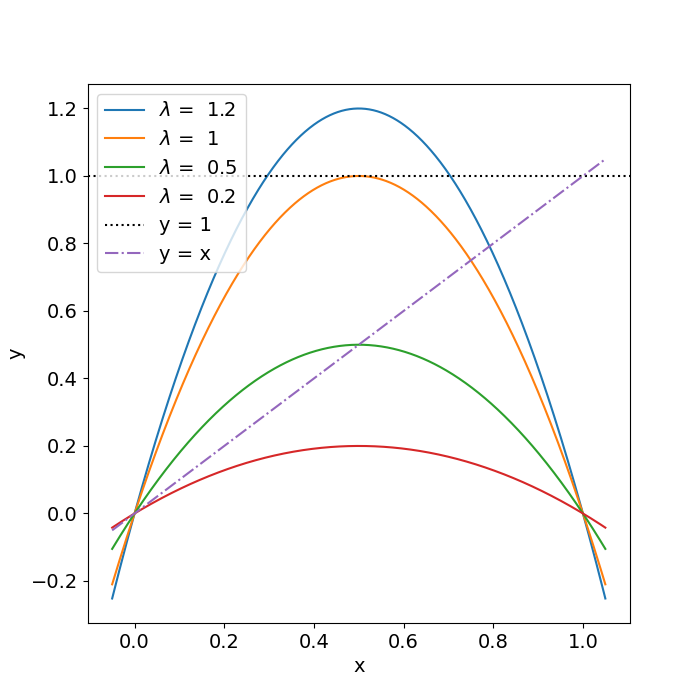
\includegraphics[width=0.7\textwidth]{./figures/logistic_map_diff_lambda.png}
	\caption{Graphs of logistic map $L_{\lambda}(x) = 4 \lambda x(1-x)$ for different $\lambda$ compared with the line $y=x$ and $y = 1$.} 
	\label{fig:logistic_map_diff_lambda}
\end{figure}


For our purpose the restriction $\lambda >0$ is applied.
Scrutinising the class of discrete logistic functions plotted in figure \ref{fig:logistic_map_diff_lambda}, some of their properties are obvious

\begin{enumerate}
	\item $\L$ is a smooth function.
	\item $\L$ concaves downwards, that is, $\L'' < 0$.
	\item $\L$ attains a unique maximum at $x = \frac{1}{2}$, and $L_{\lambda}(\frac{1}{2}) = \lambda$.
	\item When $0 \leq \lambda$ and $x$ is restricted to the domain $[0, 1]$, $\L$ is a two-to-one non-surjective (except for $\lambda = 1$) function $\L: [0,1] \rightarrow [0,\lambda]$. 
\end{enumerate}

Some sources defined the logistic map as $L'_{\lambda'}(x) = \lambda' x(1-x)$ without the constant 4. 
In this report, however, we will use equation \ref{eq_logistic}, which has the advantage that the maximum value attained by $\L$ is $\lambda$. This notation will also be consistent to the definitions of other class of functions discussed later in the report.

We can check if this model would work as expected by comparing it to its continuous counterpart 

\begin{equation}\label{eq_logistic_continuous}
	\frac{dp}{dt} = c p(x) (1-p(x)),
\end{equation}

whose unique solution with the initial condition $p(0) = \frac{1}{2}$ is 

$$
p(t) = \frac{e^{cx}}{1+e^{cx}}
$$

\begin{figure}[b!]
	\centering
	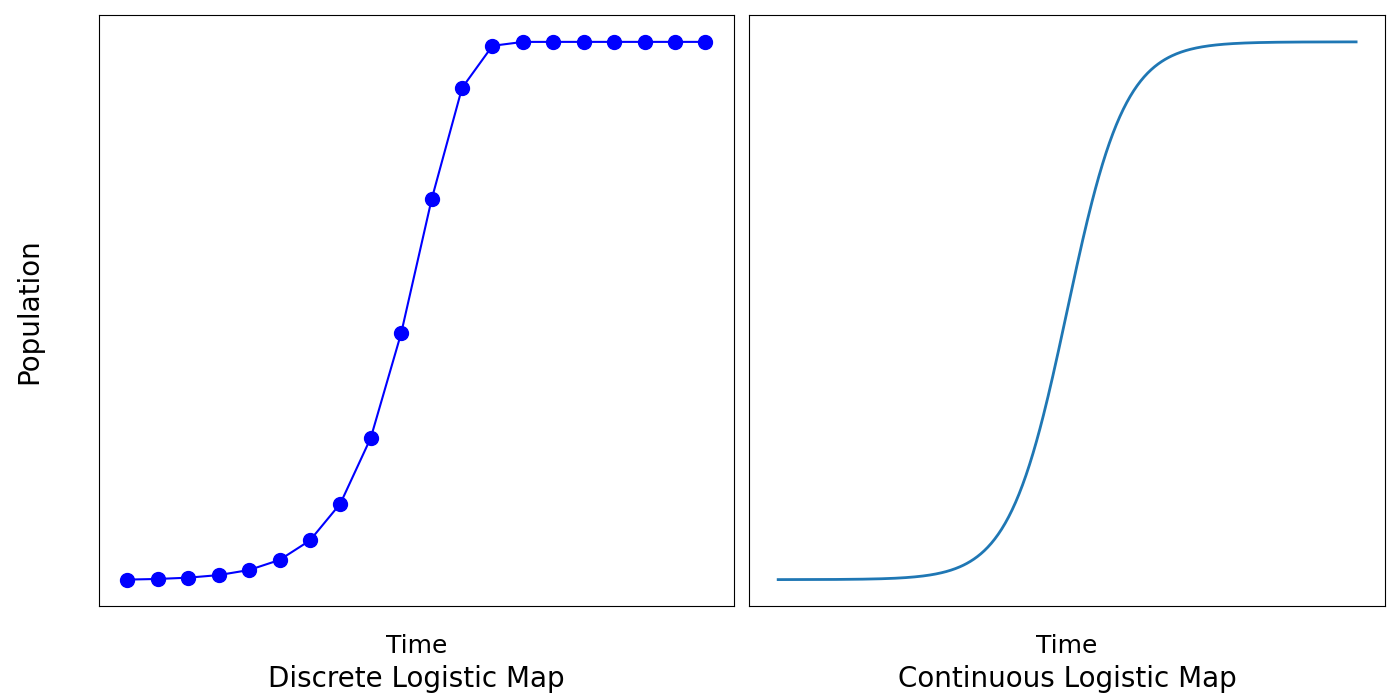
\includegraphics[width=0.8\textwidth]{./figures/con_vs_discrete_logistic_map.png}
	\caption{Discrete (left) v.s. continuous (right) logisitc map. Discrete case is modeld by $\lambda = 0.5$ and $x_0 = 0.0003$. The continuous case has $c=1$.}
	\label{fig:con_vs_discrete}
\end{figure}

The graph of these two maps are shown in figure \ref{fig:con_vs_discrete}.
The population of the discrete case was obtained by setting an arbitrary initial value, here $x_0 = 0.0003$, and the population of the next time interval was obtained by simple iteration of the logistic map, that is $x_{i+1} = L_{\lambda}(x_i)$.
For the continuous case the population at each time was obtained by solving the differential equation with initial condition.
Indeed, at least for the selected value of $\lambda$ and $c$, the population modeld by the two maps are similar.

Having settled that the discrete logistic map is indeed, at least for some values of $\lambda$, a good simplification for the already-simplified equation \ref{eq_logistic_continuous} as a model for population growth, you may wondered why bother studying such a simple equation. 
The reason is, as simple as it seems, the iteration of equation \ref{eq_logistic} gives rise to some extremely complicated dynamical systems with many surprising properities. 
These interesting dynamics are also observed in the continuous case and is the study of the next session.

% graph produced by logistic_vs_continuous_modelling_population


\section{Logistic Bifurcations}

The first step of studying logistic bifurcations is to plot it with different initial values and $\lambda$. 
For now only $0 \leq \lambda \leq 1$ and $0 \leq x_0 \leq 1$ are considered, so that $\L$ is a map from $[0,1]$ to $[0,1]$. 

% graph produced by `modelling_pop_with_diff_logistic_maps` in `graph_qc` repo
\begin{figure}[htbp]
	\centering
	\label{fig:various_iter_logistic}
	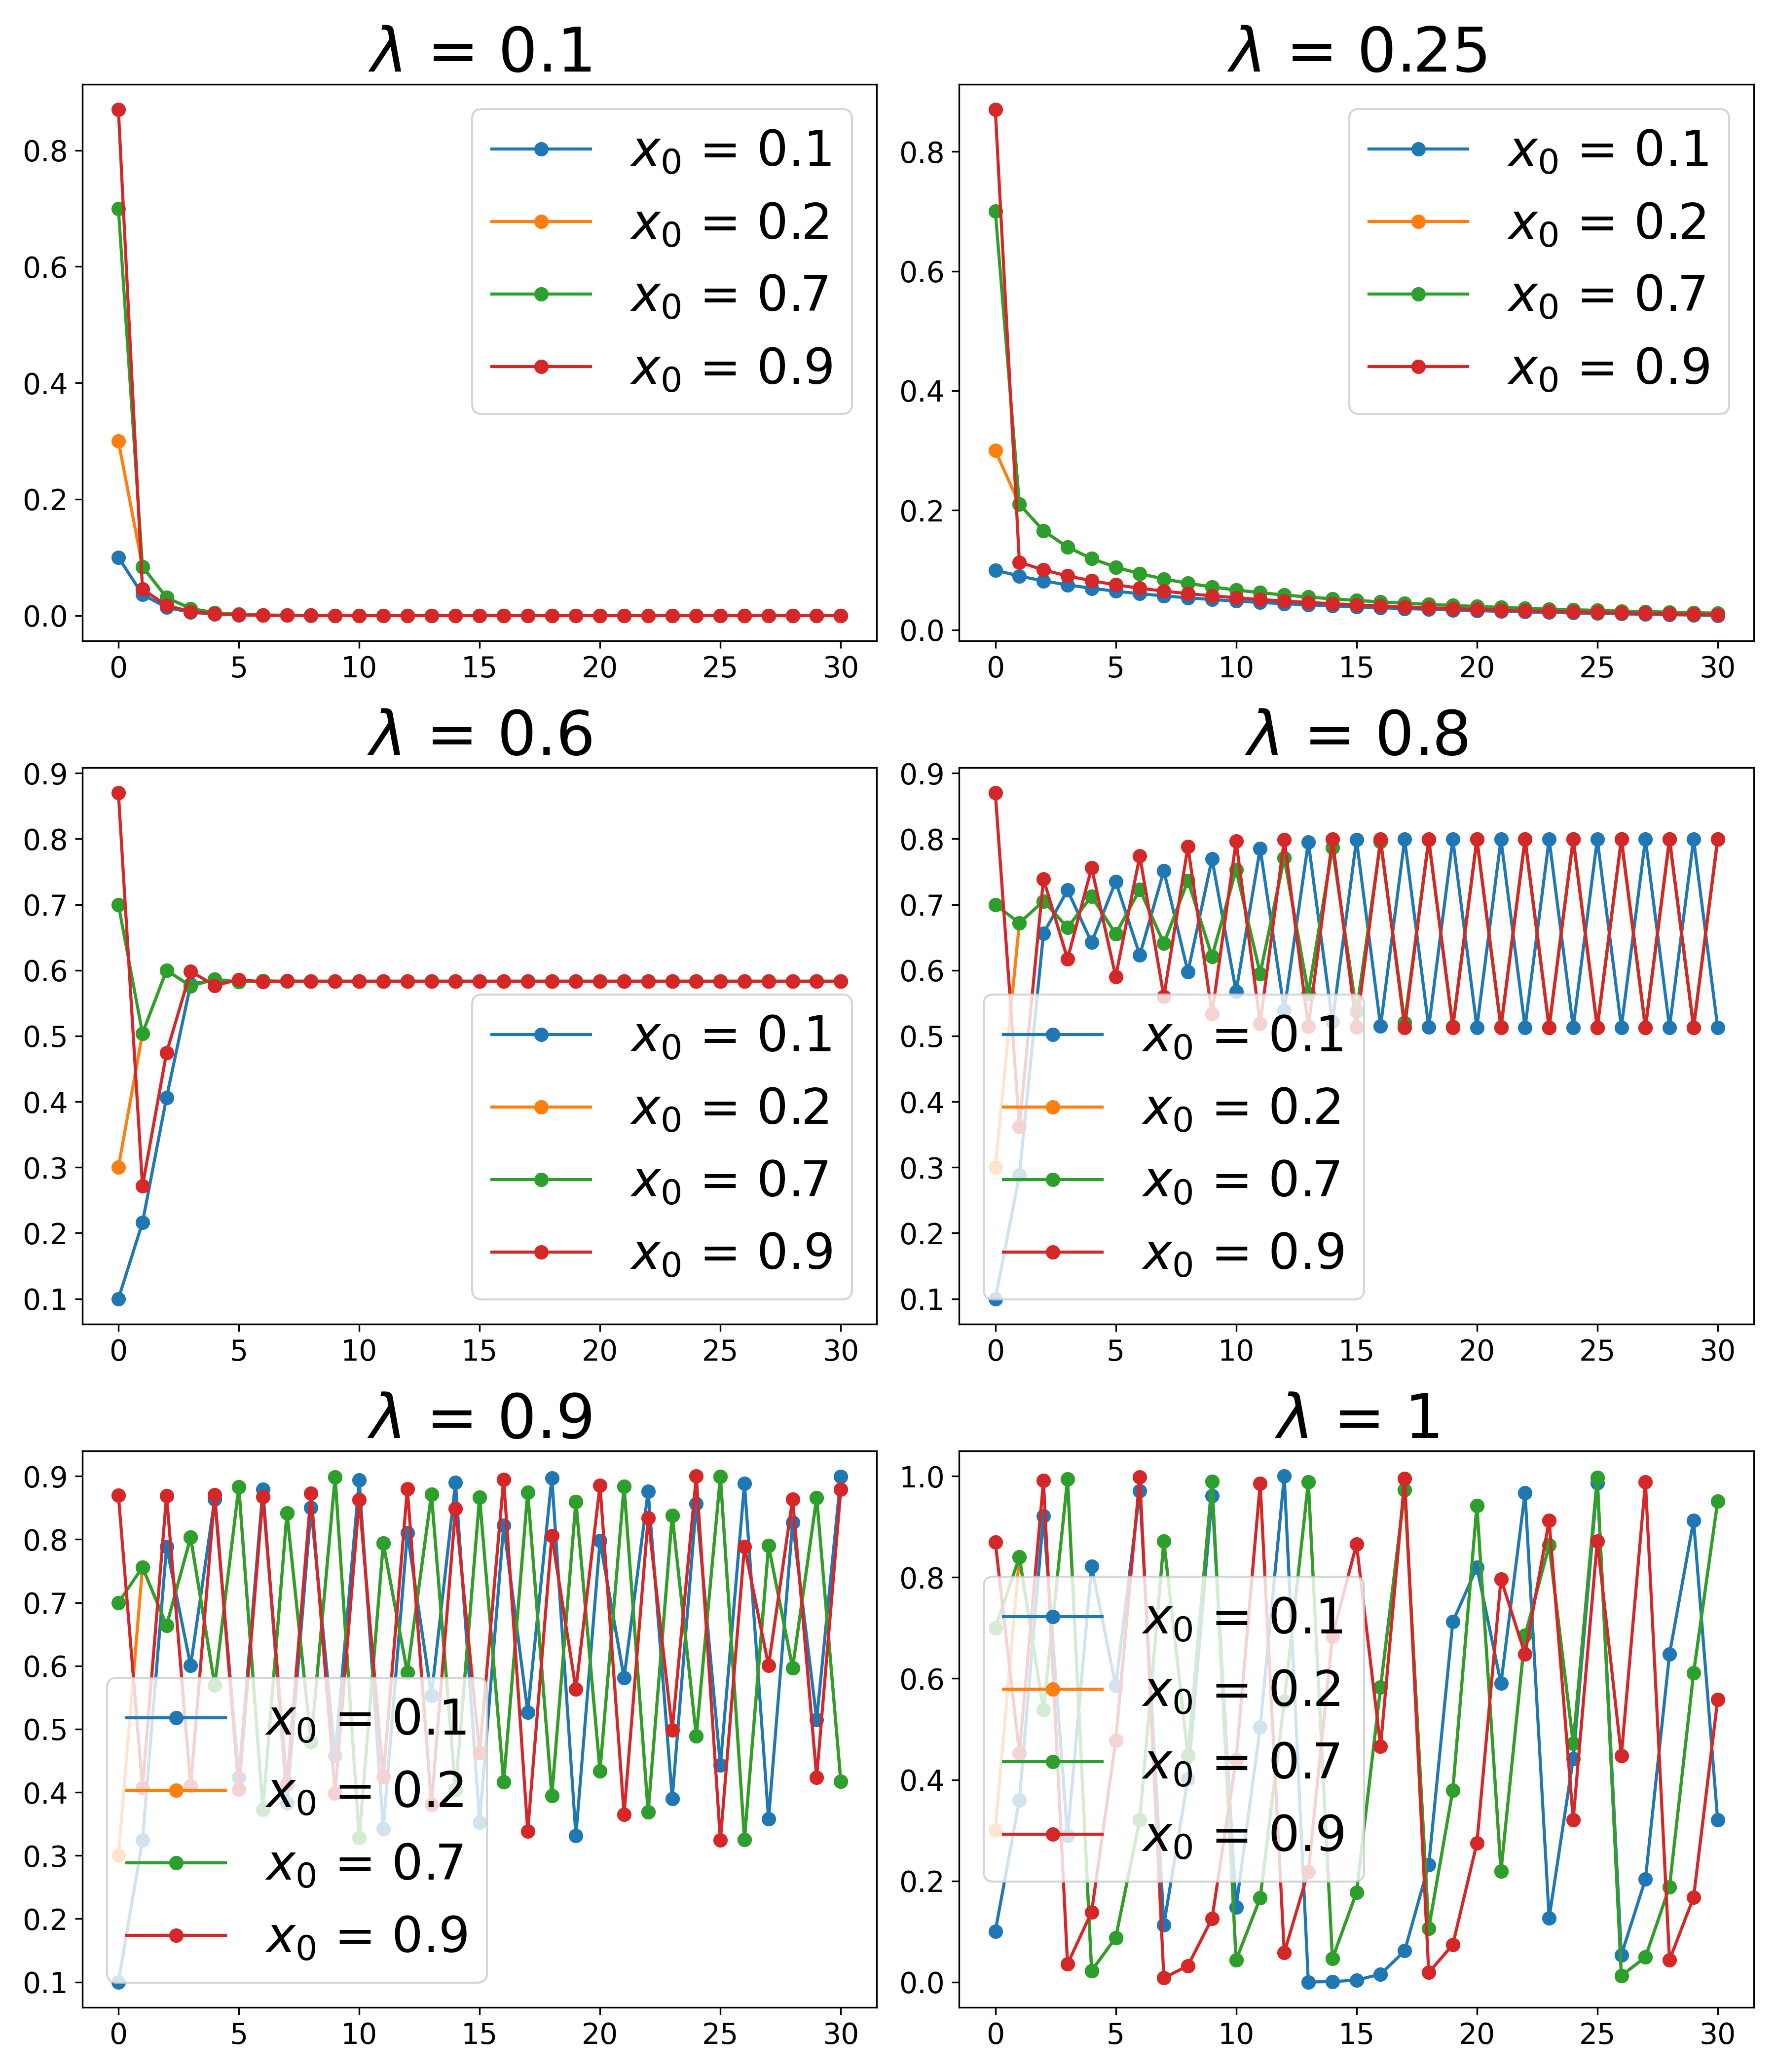
\includegraphics[width=\textwidth]{./figures/various_iterating_logistic_map.png}
	\caption{Iterating the logistic map with different initial values and $\lambda$. All graphs are produced by setting a $x_0$ and $\lambda$, and iterating $x_{n+1} = L_{\lambda}(x_n)$, and plotting all $x_n$ values respect to iteration number $n$.}
\end{figure}

There are several immediate observations upon looking at the figure \ref{fig:various_iter_logistic}.
When $\lambda = 0.1$ and $0.25$, it seems $\lim_{n \rightarrow \infty} x_n = 0$ regardless of the value of $x_0$.
For $\lambda = 0.6$, $\lim_{n \rightarrow \infty} x_n = l \neq 0$. 
(We can show that, after more tools a developped in the next sessions, $l = \frac{7}{12}$). 

When $\lambda = 0.8$, $x_n$ no longer converges, instead it seems to oscillate in a stable two orbit. When $\lambda = 0.9$ and $\lambda = 1$, it is not clear that if $x_n$ has any stable orbits or sensible patterns, and the best epithed for them would be `chaotic'.
A rigorous topological definition for chaos will be provided in the following session.

For all cases it seems like any initial condtion, $x_0$, upon iteration, will eventually tend to some common dynamical behavior depending only on $\lambda$.
The scatter plot, figure \ref{fig:logistic bifurcation overview}, is produced to capture the behavior of $x_n$ as $n \rightarrow \infty$ for $0 \leq \lambda \leq 1$. 
Two zoomed in figure around the area of bifurcation are also produced.

These pictures of bifurcation are indeed spectacular. 
There is one single stable orbit until $\lambda = 0.75$, after which a stable two cycles appears.
The two cycle bifurcated to 4 cycles, $2^3$ cycles, $2^n$ cycles, but after some threshold around $\lambda = 0.88$, there are no longer clear stable cycles and all that is left are chaos. 


\begin{figure}[htbp]
	\centering
	\label{fig:logistic bifurcation overview}
	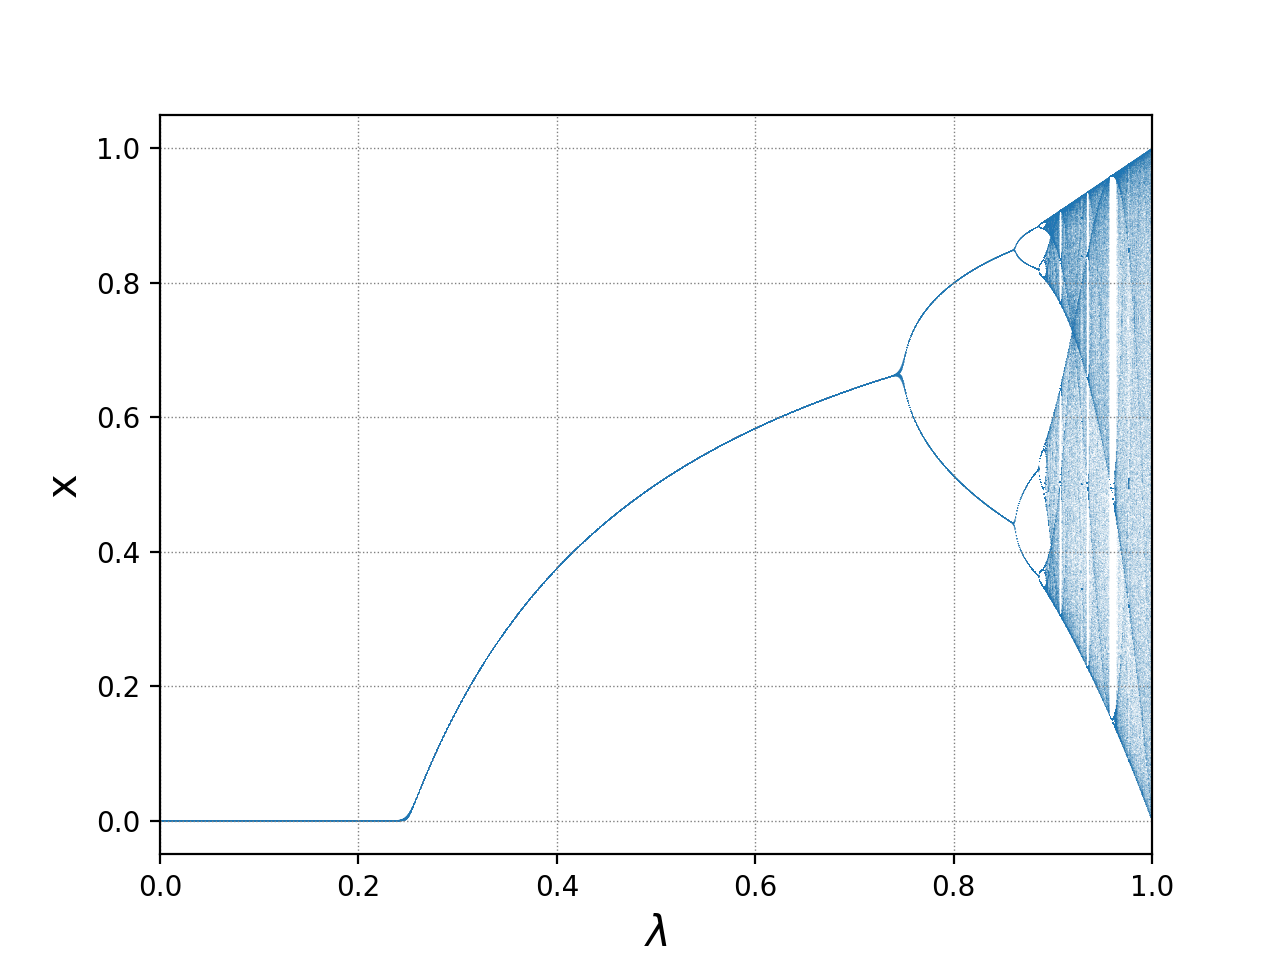
\includegraphics[width=\textwidth]{./figures/l_bifurcation_overview.png}
	\caption{For each $\lambda \in [0,1]$, $x_0$ is set to $0.5$, and the value of each iteration of $x_{n+1} = L_{\lambda}(x_n)$ was plotted at the coordinate $(\lambda, x_{n+1})$ as a faint blue dot. 
	The first 100 iteration was discarded, and 1500 iterations were plotted for each value of $\lambda$.}
\end{figure}

\begin{figure}[htbp]
	\centering
	\label{fig:logistic_bifurcation_zoom_1}
	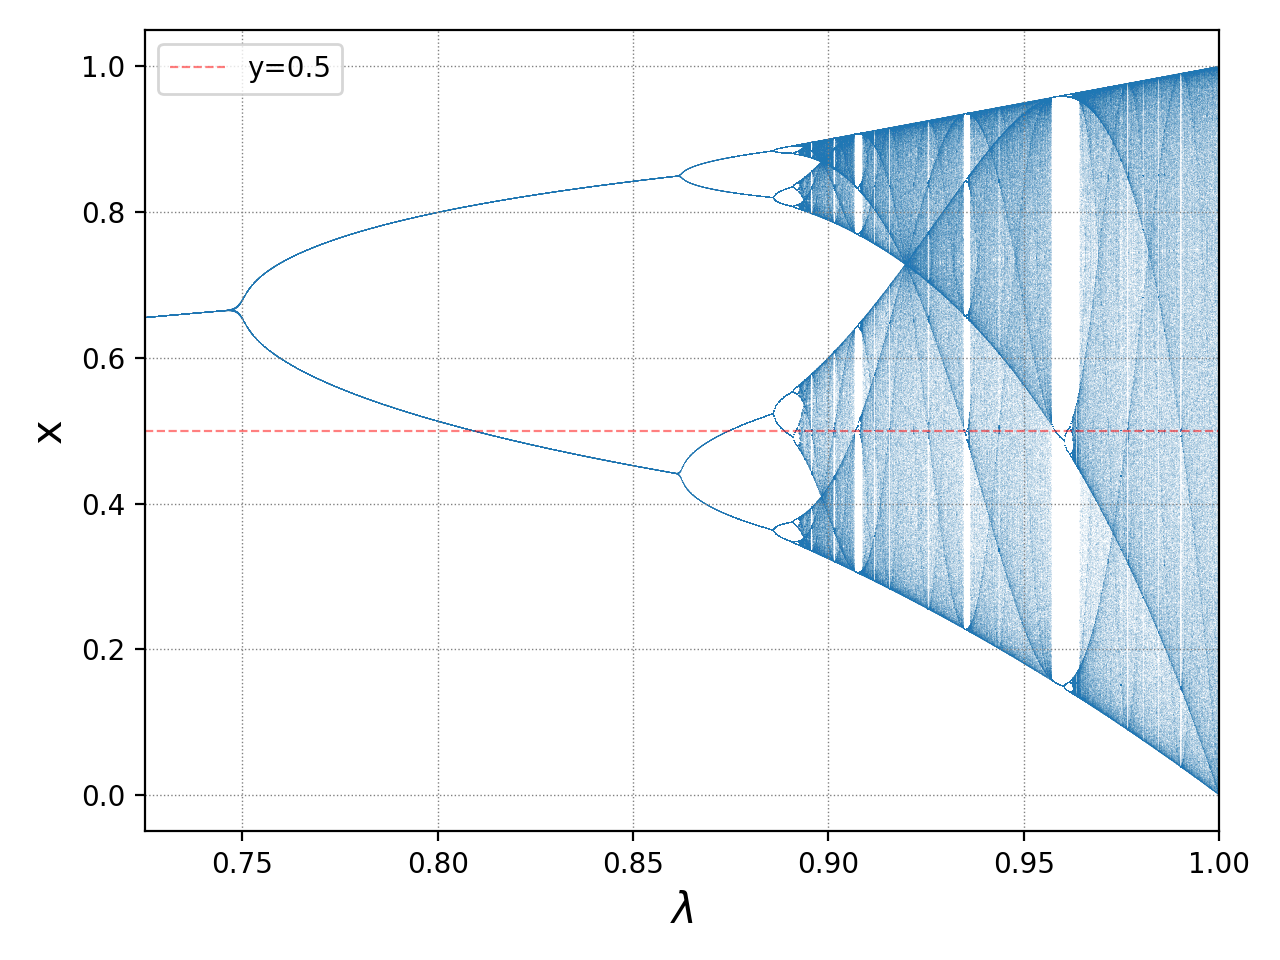
\includegraphics[width=\textwidth]{./figures/l_bifurcation_zoom_1.png}
	\caption{Zooming in the figure \ref{fig:logistic bifurcation overview} at the interval $0.5 \leq \lambda \leq 1$.}
\end{figure}

% TODO: caption non finished
\begin{figure}[htbp]
	\centering
	\label{fig:logistic_bifurcation_zoom_2}
	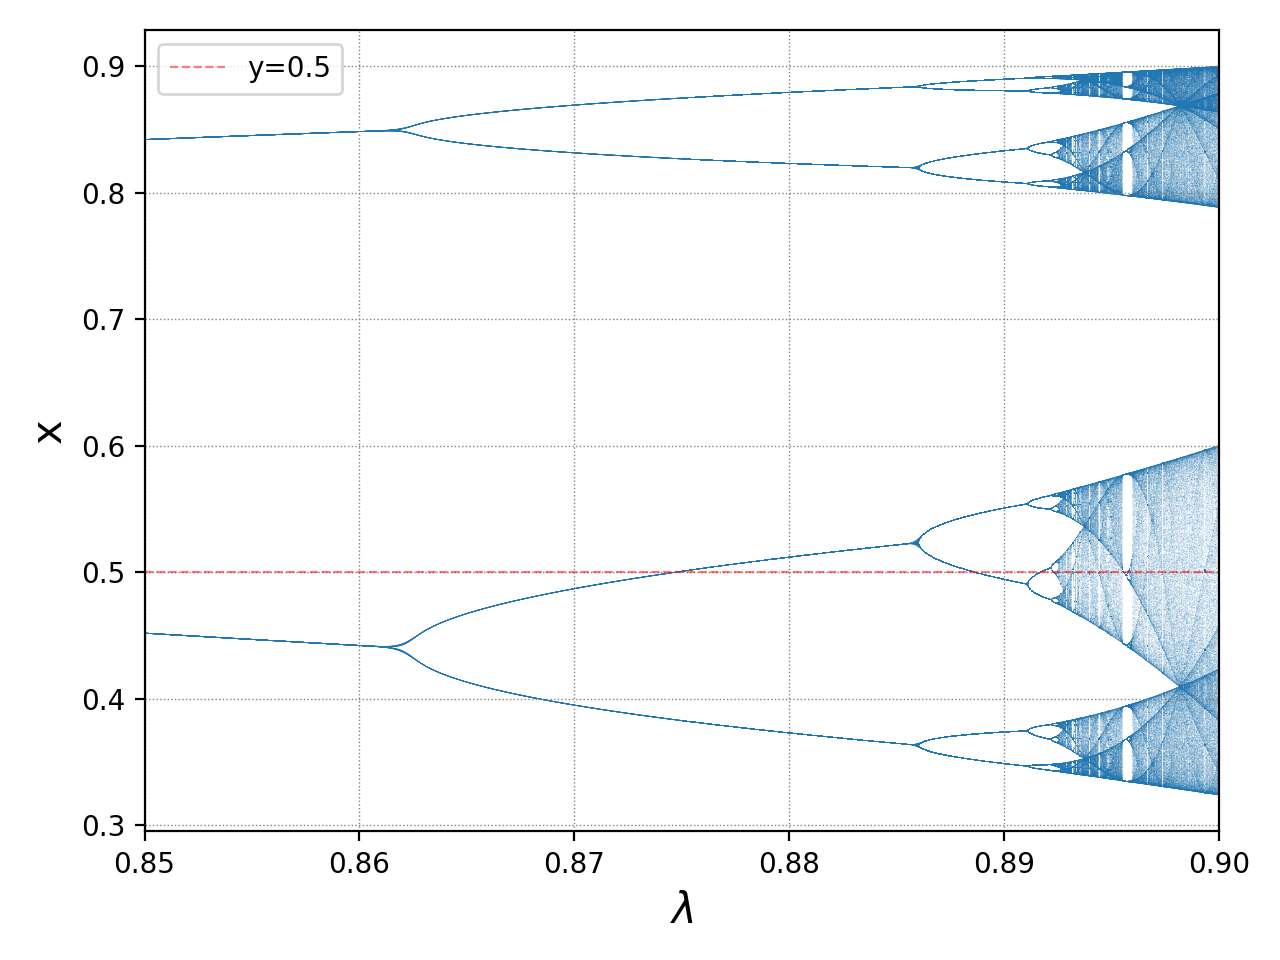
\includegraphics[width=\textwidth]{./figures/l_bifurcation_zoom_2.png}
	\caption{Zooming in the figure \ref{fig:logistic bifurcation overview} at the interval $0.5 \leq \lambda \leq 1$.}
\end{figure}

\begin{observation}[Logistic Bifurcation]\label{th:logistic_bifurcation}
	Let $f_{\lambda} = \lambda 4x(1-x) $ be the logistic function with a parameter $\lambda$, which takes value from $0$ to $1$. 
	Notice the $f_{;}$ attains the unique maximum 1 at $\mx = \frac{1}{2}$, and $f_{\lambda}(\mx) = \lambda$.
	Let $x_0 \in [0,1]$ and generate sequence of $x_i$ such that $x_{i+1} = f_{\lambda}(x_i)$.
	The behavior of $x_i$ varies as $\lambda$ increases from 0 to 1. Let $0 < B_0 < B_1 < \cdots < B_{\infty} < 1$ be the value of $\lambda$ at which the behavior of $x_i$ changes.

	\begin{enumerate}
		\item For all $0 < \lambda < B_0$, $x_i$ has a unique and stable one cycle at $x=0$.
		\item For all $B_0 <\lambda < B_1 = \frac{3}{4}$, the one cycle at $x=0$ is no longer stable, but a new stable one-cycle were developped.
		\item When $\lambda = \mx = \frac{1}{2}< B_1$, the one circle attains superstability. Define $A_1 = \mx$ .
		\item When $\lambda > B_2$, the one cycle is no longer stable. Precisely at the point when the one cycle fails to be stable, a stable two cycle appears.
		\item At some $B_2 <A_2 < B_3$ the 2 cycle enjoys superstability, and one of the value of the $2$ cycle must be $\mx$.
		\item Similar trends continue. When $\lambda > B_k$, the previous $2^{k-2}$ cycle becomes unstable and a new stable $2^{k-1}$ cycle were developped. One of the value of the cycle must be $\mx$ at some $\lambda, B_k <\lambda < B_{k+1}$, and at this point the cycle enjoys superstability.
		\item $B_{\infty} < 1$, and for most of the value after $B_{\infty}$ $x_i$ behaves. 
		\item Specifically, at $\lambda = 1$, $x_i$ has chaotic behavior defined in TODO
	\end{enumerate}

\end{observation}

\section{Single Nodal Functions Give Rise to Bifurcations}

It is very common for a mathematic model to consist, at least in parts, of iterations of some functions.
For the sake of simplicity and generosity, assume the value of our interest is $x_i$ is modelled by the simple recursive relations $f$ with the parameter $\lambda$. With appropriate rescaling, we assume moreover $x_i \in [0,1], \lambda \in [0,1]$ and $f: [0,1] \rightarrow [0,1]$:

\begin{equation}
	x_{i+1}=\lambda f(x_i)
\end{equation}
The presice definition of $f$ and $\lambda$, of course, depend on the behavior of the object in interest and is not of our relevence here.

%TODO: Is single nodal the correct term?
% TODO: add figure single nodal function
It may seem like nothing can be said by such a generalised model. However, with one more modest restriction that $f$ is single nodal, which just means the profile of $f$ is similar to figure TODO:, $x_i$ will exhibit the surprising structure of bifurcation, showing in figure (TODO: add figure)

% TODO: what is the correct term of B_1 A_1 etc?
\begin{thm}[Bifurcation]\label{th:general_bifurcation}
	Let $f_{\lambda}: [0,1] \rightarrow [0,1] $ be a single nodal function with a parameter $\lambda$, which takes value from $0$ to $1$. 
	Assume the $f_{1}$ attains the unique maximum 1 at $\mx$.
	Let $x_0 \in [0,1]$ and generate sequence of $x_i$ such that $x_{i+1} = f_{\lambda}(x_i)$.
	The behavior of $x_i$ varies as $\lambda$ increases from 0 to 1. Let $0 < B_0 < B_1 < \cdots < B_{\infty} < 1$ be the value of $\lambda$ at which the behavior of $x_i$ changes.

	\begin{enumerate}
		\item For all $0 <\lambda < B_1$, $x_i$ has a unique and stable one-cycle
		\item When $\lambda = \mx < B_1$, the one circle attains superstability precisely at $\mx$. Define $A_1 = \mx$ .
		\item When $\lambda > B_2$, the one cycle is no longer stable. Precisely at the point when the one cycle fails to be stable, a stable two cycle appears.
		\item At some $B_2 <A_2 < B_3$ the 2 cycle enjoys superstability, and one of the value of the $2$ cycle must be $\mx$.
		\item Similar trends continue. When $\lambda > B_k$, the previous $2^{k-2}$ cycle becomes unstable and a new stable $2^{k-1}$ cycle were developped. One of the value of the cycle must be $\mx$ at some $\lambda, B_k <\lambda < B_{k+1}$, and at this point the cycle enjoys superstability.
		\item $B_{\infty} < 1$, and for most of the value after $B_{\infty}$ $x_i$ behaves. 
		\item Specifically, at $\lambda = 1$, $x_i$ has chaotic behavior defined in TODO
	\end{enumerate}

\end{thm}

Here is the precise definition for a function to be single nodal:

% TODO: is a circle signle nodal? for all $\lambda$ the cicle has exactly on stable one-cycle. 
% TODO: are there more examples like the circle? Or are there more examples of similar function that only exhibit finite Bifurcations?

\begin{defn}
	A function $f: [0,1] \rightarrow [0,1]$ is single nodal if 
	\begin{enumerate}
		\item $f$ is piecewise $C^2$, that is, doubly differentiable with continuous second derivative
		\item $f$ has a unique and differentiable maximum attained at $f(\mx) = 1$ and $f'$ is continuous at $\mx$.
% TODO: Do we need the condition that f has no other local maximum?
		\item $f(x) > 0$ and $f(1) = f(0) =0$
		\item $f(x)$ concave downwards, that is $f'' < 0$.
	\end{enumerate}

	This definition is modified from appendix A of Feigenbuam's paper \cite{F1}.
\end{defn}

Although theorem \ref{th:general_bifurcation} may seem extremely bold in claim, 


\chapter{Chaos With Rigour}
For the entirety of this report we have been loose on using the term chaotic.
This chapter attempts to remedy this and give some rigorous treatment of chaos using tools in topology and analysis and provides proof for some theorems which we relied heavily for the rest of the report.

\section{Introduction to one dimensional dynamics}

The term \emph{dynamical system} describes a branch of mathematics that studies a process which evolves over time \cite{Devaney_green_book_chaos_definition}.
Most of this report concentrates on the one dimensional system consists of sequence of number $x_0, x_1, \cdots$, where $x_0$ is some arbitrary starting point and $x_{n+1} = f(x_n)$, where $f$ is a function of interest. 

Our first definition is fixed point.

\begin{defn}[Fixed Point]
	Assuming we have a iterated dynamical system $x_{i+1} = f(x_i)$. 
	The fix point of $f$ is a point $x^*$ such that $f(x^*) = x^*$. 
	That is, the fixed points are the solution to the equation $f(x) = x$.
\end{defn}

Fixed points are like sinks in the dynamical system. 
If for some $c$ there exists a $n$ such that $f^n(c) = x^*$, $c$ will stay at $x^*$ forever. 
Our intuition tells us that the fixed points shall determine, at least in parts, the properties of the dynamical system.
In deed, for some dynamical system $f = x$ for all $x \in I$, where $I$ is some interval, what takes place in that interval would not be so interesting.

Many interesting dynamical system have infinitely many fixed point, but the set of fixe point is of measure zero, meaning if picking any point in the interval at random, there is a zero chance that it is a fixed point.
Two traditional examples for a set of measure zero are rational points and cantor set on the real axis. 

Given a fixed point, it is natural to ask what are the behaviors of the dynamical system nearby it.
Will nearby points converge to it, or diverge from it?
It turns out both are simplifications, and the proper description of the behavior is that it will either be a \emph{stable} fixed point or an \emph{unstable} one. 

Here is the rigorous definition of stability, attributed to the renowned Russian mathematician Aleksandr Mikhailovich Liapunov \cite{lyapunov}.

\begin{defn}[Stable fixed point]
A fixed point $x^*$ is stable if for all $\epsilon$ there exists a $\delta$ such that 
$$
	|f^n(x) - f^n(x^*)| < \epsilon \text{ for } n = 1,2, \cdots 
$$
whenever $|x - x^*| < \delta$.
Here $f^n$ denotes the composition of $f$ $n$ times.
\end{defn}

The intuition for the definition is that if $x$ is close enough to a stable fixed point $x^*$, it will stay close to it forever. 
It does not imply, however, all $x$ close to $x^*$ will converge to it.
The classical example for 1-dimension case is the identity map $f(x) = x$. 
All points are stable fixed points, but no points in a neighbourhood of the fixed point converges to it, except itself.

Considering the above example, we can define a stronger sense of stability called asymptotic stability.

\begin{defn}[Asymptotic Stability]
	A fixed point $x^*$ is asymptotically stable if it is stable and there exists a $\delta$ such that 
	$$
		\lim_{n \rightarrow \infty} f^n(x) = x^* \text{ whenever } |x - x^*| < \delta
	$$
\end{defn}

Upon settlement of this definition, the following theorem is immediate.

\begin{thm}[Stable and unstable fixed point]\label{th:_stable_unstable_fixed_point}
	If $x^*$ is a fixed point of a two time differentiable function $f$ and $|f'(x^*)| < 1$, $x^*$ is a  asymptotic stable fixed point.
	If $|f'(x^*)| > 1$, $x^*$ is unstable.
	If $|f'(x^*)| = 0$, $x^*$ may be stable or unstable.
\end{thm}

\begin{figure}
	\centering
	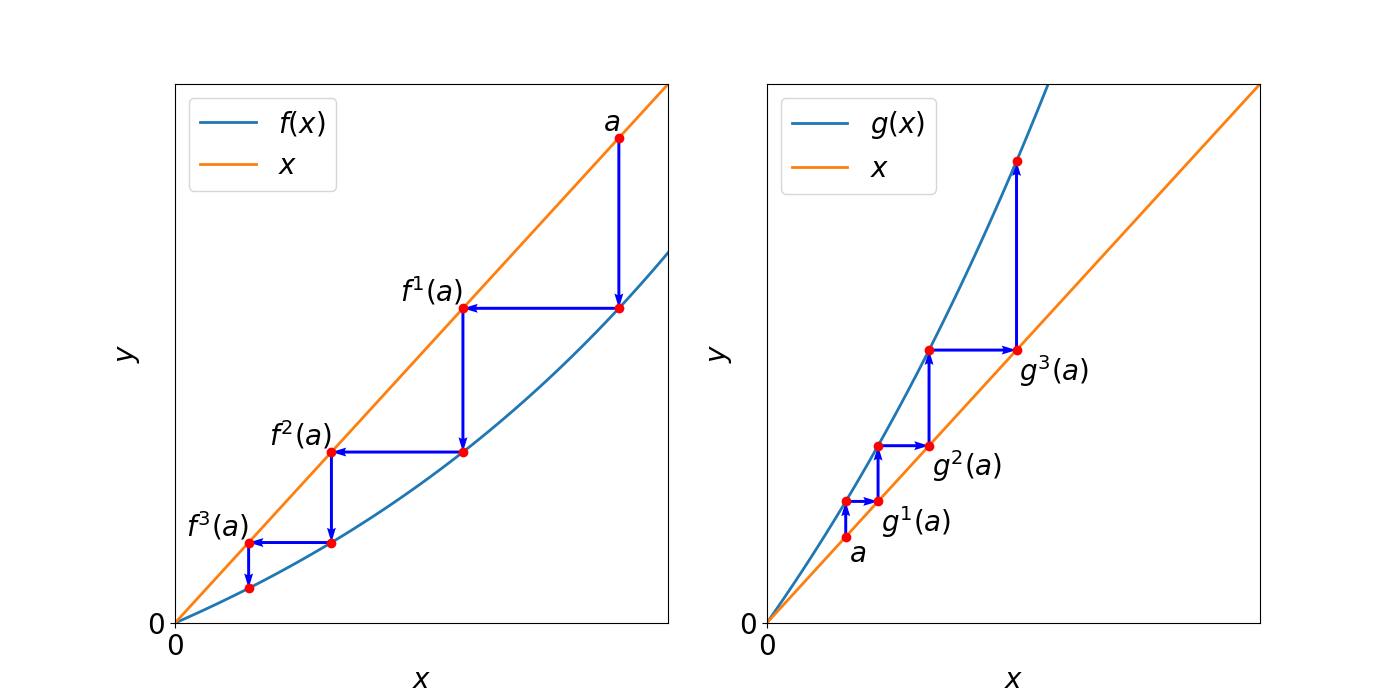
\includegraphics[width=\textwidth]{./figures/stable_and_unstable_fixed_point.png}
	\caption{An illustration of theorem \ref{th:_stable_unstable_fixed_point}.
	The figure on the left shows function $f(x) = 0.4 e^x - 0.4$, which has a stable fixed point at $x^* = 0$. 
	The figure on the right shows function $f(x) = 1.3 e^x - 1.3$, which has an unstable fixed point at $x^* = 0$.}
	\label{fig:stable and unstable fixed point}
\end{figure}

Figure \ref{fig:stable and unstable fixed point} is an illustration of this theorem.
To prove this theorem is a regular exercise using Taylor expansion. 

Assuming $x^*$ is a fixed point of the iterated map $f$ whose Taylor expansion is
$$f(x) = f(x^*) + f'(x^*) (x - x^*) + O(x^2)$$

For any $\delta$ let is evaluate $f(x^* + \delta)$.
Since $x^*$ is a fixed point,
 $f(x^*) = x^*$, and
 $f(x^* + \delta) - f(x^*) = f'(x^*) \delta + O(x^2)$. 
For small enough $\delta$ we can ignore all the terms of degree higher than $2$, and the above equation states $x^*+ \delta$ will eventually converge to $x^*$ if $|f'(x^*)| < 1$, and diverge if $|f'(x^*)| > 1$.

This theorem, though simple, is powerful and is a fundamental part for any rigorous approach of iterated dynamical systems and is also used multiple times in this report (such as in the proof of \ref{th:logistic_bifurcation}). 
As a result, hereby we give another proof using only the classic mean value theorem and $\epsilon-\delta$ definition of limit.

\begin{proof}[Proof of Theorem \ref{th:_stable_unstable_fixed_point}]
	Without loss of any generality we can assume that the stable fixed point is $0$, meaning $f(0) = 0$. 
	If the function $f^*$ has stable point not at $0$ but at $x^*$, we can always investigate the function $f(x) = f^*(x+x^*) - x^*$. 
	
	If for a neighbourhood of $0$ $f' = 0$, we are done, as by mean value theorem $f = 0$ in this neighbourhood, and every $x$ in this neighbourhood converges to $0$ after one iteration.

	If $f' \neq 0$, since $f'$ is continuous, there exists an interval around $0$ such that $f'(x)$ is either strictly positive or strictly negative in this interval (depending on the sign of $f'(x)$), and, since $|f'(0)| < 1$, we can further restrict the interval such that $|f'(x)| < c < 1$. 
	Label this interval as $I$. 
	Notice by construction, this interval is a neighbourhood of $0$, so it must contain $0$.
	
	First, consider $0 < f'(x) < c < 1$ for $x \in I$. 
	For any point $a<0$ and $a\in I$,  $f(a)$ must be small than $0$. 
	Otherwise, the function $f$ will be overall decreasing in the interval $(a, 0)$, and by mean value theorem there will be a point $a^*$ such that $a < a^* < 0$ and $f'(a^*) = \frac{f(a) - f(0)}{a - 0} = \frac{f(a)}{a} < 0$, which is impossible.

	Since $f(a) < 0$, we can further shows that $f(a) > a$. 
	If $f(a) < a$ by mean value theorem there is some point $a^* \in (a, 0)$ such that $f'(a^*) = \frac{f(a) - f(0)}{a - 0} = \frac{f(a)}{a} > 1$, which also impossible.

	As a result the sequence $a, f(a), f^2(a), \cdots$ is monotonically increasing and bounded above by $0$, and by the completeness of the real number it must converge to some number. 
	Assuming it converges to $l < 0$. 
	Let us pick a point $a$ in the interval $(\frac{l}{c}, l)$. 
	That is, $a > \frac{l}{c} \implies \frac{l}{a} > c$ and $f(a) < l$.
	Notice 
	$$
	\frac{f(0) - f(a)}{0 - a} = \frac{f(a)}{a} > \frac{l}{a} > c
	$$
	Where $c$ is the constant defined above such that in the whole interval $|f'(x)| < c$.
	By mean value theorem, there exists a point $b$ in the interval $(a, 0)$ such that $f'(b) = \frac{f(a)}{a} > c$, which is a contradiction.

	All of other cases ($a > 0, f'(0) < 1$) can be proved similarly.
\end{proof}

This theorem does not apply if the derivative of a function at a fixed point is $\pm 1$.
If such is the case the fixed point may be stable or unstable, or it may exhibit more interesting behaviors.
For example, the function $f(x) = e^x - 1$ has a fixed point at $0$.
All $x$ smaller than $0$ will converge to $0$ upon iterations, while all $x$ larger than $0$ will diverge to infinity.

\section{Devaney's Definition of Chaos}

We have used the term chaotic serveral times in this report without rigorous definition. 
In this session we will settle this problem.

One intuition is that every point in the chaotic system can be ``mixed'' with any other point after some time interval. 
This is captured by topological transitivity.
\begin{defn}[Topologically Transitive]
	Let $J$ be a set with a topology.
	The function $f: J \rightarrow J$ is topologically transitive, if for all non-empty open sets $U_1, U_2 \in J$, there exist $k \in \bb{N}$ such that $f^k(U_1) \cap U_2 \neq \varnothing$. 
	Here $f^k$ denotes the composition $\underbrace{f \circ f \cdots \circ f}_{k \text{ times}}$
\end{defn}

The second intuition for chaos is that a small change in the initial condition can lead to a large change in the final condition. 
Liapunov exponent is a quantitative measure of this, but here we present another analytical definition, which is sensitive dependence on initial condition. This term is coined by Ruelle \cite{Ruelle-1978}.
\begin{defn}[Sensitive Dependence on Initial Condition]
	Let $J$ be a metric space with the metric $d: J \times J \rightarrow \bb{R}$.
	$f: J \rightarrow J$ has sensitive dependence on initial condition if there exists some $\delta > 0$ such that for all $x \in J$ and any neighbourhood $X$ containing $x$, there exists $y \in X$ and $n \in \bb{N}$ such that $d(f^n(x), f^n(y)) > \delta$.
\end{defn}

Maybe the most striking fact about chaotic system that, although seemingly chaotic, some order still remains.
Since chaos tent to mix every points together, it is natural that some points will return to their original position after certain iterations.
Although we may simply decree periodic points are infinite, using topology we can state a stronger and more precise definition, that is, the periodic points are dense.

Of course. a point $x$ is a period of period $k$ if $f^k(x)=x$, and dense here is in sense of topology.

Therefore we have arrived at the following definition.

\begin{defn}[Chaos, Devaney's Definition]\label{def:Devaney_definition_for_chaos}
	Let $V$ be a metric space.
	A function $f: V \rightarrow V$ is chaotic if 
	\begin{enumerate}
		\item the set of periodic points are dense in $V$,
		\item $f$ is topologically transitive,
		\item $f$ has sensitive dependence on initial condition. 
	\end{enumerate}
	
\end{defn}


The definition here is attributed to Devaney \cite{Devaney_green_book_chaos_definition}. 
The first two requirements are purely topological, while the last one requires a metric. 
While in most circumstances topological properties are more generalised than the metric properties, here, surprisingly, as long as $V$ is a metric space (which is part of the assumption), the first two implies the third\cite{Banks}. 
As a result, we only need to check the first two conditions to determine if a function is chaotic.

\begin{thm}[Criterion For Chaotic Function]
	Let $V$ be a metric space. 
	Function $f: V \rightarrow V$ is chaotic as defined in \ref{def:Devaney_definition_for_chaos}
	if and only if its the periodic points are dense $V$ and it is topologically transitive,
\end{thm}

% TODO: Say more about doubling map. 
% TODO: graph, say more in introduction, etc?
% The doubling map is topologically transitive to the map in $S^1$

\begin{example}\label{ex_doubling_map}
	Recall the doubling map $f: [0,1) \rightarrow [0,1)$
	\begin{equation}\label{eq:doubling_map}
	f(x) = 
		\begin{cases}
			2x &\text{ if } 2x < 1 \\
			2x -1 &\text{ if } 2x > 1
		\end{cases}
	\end{equation}
	% TODO: more explanation
	This map can also be regarded as doubling the angles on the unit cycle: $g: S^1 \rightarrow S^1$ given by $ g(\theta) = 2 \theta$.
	
	The doubling map is \textit{chaotic}.

	All non-zero rational points $\frac{p}{q} \in [0,1)$ with odd denominater are periodic points for $f$. 
	The set of these points are dense.
	To show the periodicity, note the images of $\frac{p}{q}$ under repetitive applications of $f$ are $\frac{p}{q}, \frac{2p}{q}, \cdots, \frac{2^k p}{q}, \cdots$.
	We can regard all the numerators as the equivalence classes module $q$.
	Since this sequence is infinite and there are only finitely many possibilities for the numerators, some of the numerators must coincide. Let them be $2^k p$ and $2^{k'} p$. 
	Without loss of generacity let $k > k'$, and
	$$
	2^k p \equiv 2^{k'} p \mod q \implies 
	2^{k-k'} p \equiv p \mod q \text{ (as $q$ is odd)},
	$$
	which measn $f^{k-k'}(\frac{p}{q}) = \frac{p}{q}$, i.e., $\frac{p}{q}$ is a point of period $k - k'$.

	To show $f$ is topologically transitive is even easier. 
	For any non-empty open set $U \in [0,1)$, by definition there exists an open interval $J = (x, x+ \delta) \subseteq U$. 
	$J$ has diameter $\delta$, $f(J)$ has diameter $2 \delta$, and $f^k(J)$, $2^k \delta$. 
	Since the length of $[0,1)$ is $1$, after some finite iteration $f^k(J)$ would covers all of $[0,1)$ and intersect any other open sets.

	By generalising this proof it is clear any maps in the form 
	$$
	g: S^1 \rightarrow S^1; g(\theta) = r \theta, r \in R
	$$
	are chaotic.
\end{example}

\section{Topological Conjugacy}

To prove the doubling map is chaotic is a gentle exercise. 
To directly find the points of periodicity and prove that a general function is topologically transitive is difficult.
Instead, we can circumvent these challenges by exploiting certain topological properties called topological conjugacy.

\begin{defn}[Topological Conjugacy]
Funcitons $f: X \rightarrow X$, $g:  Y \rightarrow Y$ are topologically conjugate if there exist a homeomorphism $\phi: X \rightarrow Y$ such that 
$\phi \circ f = g \circ \phi$,
i.e, the following diagram commutes.
\begin{center}
    \begin{tikzcd}
        X \arrow[r, "f"] \arrow[d, "\phi" swap] & X \arrow[d, "\phi"] \\
        Y \arrow[r, "g"] & Y
    \end{tikzcd}
\end{center}

The maps $f,g$ are semiconjugate if there exists a continuous surjection, $\psi$ such that $\psi \circ f = g \circ \psi$.
\end{defn}

% TODO: Shall we introduce a notation for topological conjugacy? 
% no notation is provided by Devaney or Wikipedia

To rephrase a definition, $f,g$ are conjugate if there exists and homeomorphism $\phi$ such that $f = \phi^{-1} \circ g \circ \phi$.
So $f^{n} = \phi^{-1} \circ g^{n} \circ \phi$; that is $f^n$ is conjugate to $g^n$.

Topological conjugacy is an equivalence condition. 
$f$ is conjugate to itself by identity map. 
$\phi \circ f = g \circ \phi$ implies $f \circ \phi^{-1} = \phi^{-1} \circ g$, so $g$ is also conjugate to $f$.
At last we need to prove transitivity, which is illustrated in the following scheme
\begin{center}
    \begin{tikzcd}
        X \arrow[r, "f"] \arrow[d, "\phi" swap] & X \arrow[d, "\phi"] \\
        Y \arrow[r, "g"] \arrow[d, "\phi'" swap] & Y \arrow[d, "\phi'"] \\
        Z \arrow[r, "h"] & Z \\
    \end{tikzcd}
\end{center}
If $f$  is conjugate to $g$ via $\phi$, and $g$ is conjugate to $h$ via $\phi'$, $\phi' \circ \phi \circ f = \phi' g \circ \phi = h \circ \phi'' $, which means $f$ is conjugate to $h$ via $h' \circ h$. 



Topological semiconjugacy only requires a continuous surjection, $\psi$, such that $\psi \circ f = g \circ \psi$. 
As $\psi$ may not have inverset semiconjugacy can not be an equivalence condition.
Nevertheless, if $f$ is semiconjugate to $g$, so is $f^{k}$ to $g^{k}$ for any $k \in \bb{N}$. 
This is because 
$$
	\psi \circ f\circ \cdots \circ f = g \circ \psi \circ f \cdots \circ f = \cdots = g^k \circ \psi
$$

 % TODO: verify this is true
If $f$ is conjugate to $g$, necessarily $f$ and semi-conjugate to $g$ and $g$ is semiconjugate to $f$. 
However, if $f$ is semiconjugate to $g$ and $g$ is semiconjugate to $f$, $f$ is not necessarily conjugate to $g$. 

Chaotic behaviors are \emph{preserved} by conjugacy.


\begin{thm}[Semiconjugacy preserves Chaos]\label{th_semicong_chaos}
	If $f$ is semiconjugate to $g$ and $f$ is chaotic, $g$ also is.
\end{thm}
% TODO: can g chaotic implies f also is if f is semiconjugate to g?
% FIND counter example

\begin{proof}
	Let $f: X \rightarrow X$, $g:  Y \rightarrow Y$, and let $\psi$ be the promised continuous surjection such that
	$\psi \circ f = g \circ \psi$. 
	Since $\psi$ is conituously surjective, for any non-empty open set $M \in Y$, $\psi^{-1}(M)$ is an non-empty open set in $X$.

	Let us first prove that the set of periodic points of $g$ is ddense.
	For any $x$ such that $f^k(x) = x$, notice that $g^k \circ \psi (x) = \psi \circ f^k (x) = \psi(x)$. 
	This means, if the set of periodic points of $f$ is $X$, $\psi(X)$ is a sub set of the set of periodic point of $g$.

	For the sake of contradiction assuming $\psi(X)$ is not dense in $Y$. 
	This means there is a open set $M \subset Y$ such that $M \cup \psi(X) = \emptyset$.
	The preimage $\psi^{-1}(M)$ is an non-empty open set of $X$, and by assumption, it does not contains any periodic points of $f$, which is a contradiction.

	To prove that $g$ is topologically transitive, consider any non-empty open set $M, N \in Y$, and $\psi^{-1}(M), \psi^{-1}(N)$ are non-empty open set in $X$. 
	By assumption there exists some $k$ such that $f^k(\psi^{-1}(M)) \cap f^k(\psi^{-1}(N)) \neq \emptyset$, this means 
	\begin{align*}
		g^k(M) \cap g^k(N) = \psi \circ f^k(\psi^{-1}(M)) \cap \psi \circ f^k(\psi^{-1}(N)) \\
		\subset \psi( f^k(\psi^{-1}(M)) \cap  f^k(\psi^{-1}(N))) \neq \emptyset
	\end{align*}
\end{proof}

Since conjugacy impies semi-conjugacy on both directions, we have the following important proposition.

\begin{prop}[Conjugacy Class share chaotic behavior]\label{prop_conj_chaos}
	If $f$ is conjugate to $g$, $f$ is chaotic if and only if $g$ is chaotic.
\end{prop}

There are abundant examples of topological conjugacy.

\begin{example}
	In an open interval $[-\epsilon_1, \epsilon_2] \in \bb{R}$,
	$f: [-\epsilon_1, \epsilon_2] \rightarrow [-\epsilon_1, \epsilon_2]$
	is conjugate to 
	$g: [-\epsilon_1 + a, \epsilon_2 + a] \rightarrow  [-\epsilon_1 + a, \epsilon_2 + a]$
	where $g(x)= f(x -a) + a$ via $\phi(x) = x + a$.

	For a concrete example, consider the map 
	$f: [0,1] \rightarrow [0,1]$
	defined as $f(x) = 4x(1-x)$,
	which is conjugate to 
	$g(x): [-\frac{1}{2}, \frac{1}{2}] \rightarrow [-\frac{1}{2}, \frac{1}{2}]$
	defined as $g(x) = -4x^2 + \frac{1}{2}$ 
	through $\phi(x) = x -\frac{1}{2}$, i.e., $ \phi \circ f=  g \circ \phi$.
\end{example}

\begin{example}
	For closed interval $[-\epsilon_1, \epsilon_2] \in \bb{R}$. 
	$f: [-\epsilon_1, \epsilon_2] \rightarrow [-\epsilon_1, \epsilon_2]$
	is conjugate to 
	$g: [-\frac{\epsilon_1}{a}, \frac{\epsilon_2}{a}] \rightarrow [-\frac{\epsilon_1}{a}, \frac{\epsilon_2}{a}]$
	where $g(x)= \frac{1}{a}(ax)$ via $\phi(x) = ax$.


	As another concrete example, the map $f: [0,1] \rightarrow [0,1]$
	defined as $f(x) = -4x^2 + \frac{1}{2})$,
	is conjugate to 
	$g(x): [-1, 1] \rightarrow [-1, 1]$
	defined as $g(x) = 2x^2 - 1$
	through $\phi(x) = -2x$.
\end{example}

\begin{example}
	Consider the doubling map $f: [0,\pi) \rightarrow [0, \pi)$ defined thus: 
	$$
	f(\theta) = 
		\begin{cases}
			2 \theta &\text{ if } 2x <  \pi \\
			2 \theta - \pi &\text{ if } 2x > \pi
		\end{cases}
	$$
	
	This map is doubling the angle of the unit circle.

	$f$ is semi-conjugate to $g: [-1, 1] \rightarrow [-1, 1]$ defined as $g(x) = 2x^2 - 1$ through $\cos(x)$.

	Example \ref{ex_doubling_map} shows that the doubling map is chaotic, so is $g$.
\end{example}

\begin{example}\label{ex_logistic_and_doubling}
	The above 3 examples shows that the doubling map is semi-conjugate to the logistic map $L_1(x) = 4x(1-x)$.
\end{example}

\begin{example}\label{ex:logistic and tent}
	The logistic map $L_1(x) = 4x(1-x)$ in the interval $[0,1]$ is topologically conjugate to the tent map defined as 
	\begin{equation}
		f(x) = 
		\begin{cases}
			2x   &\text{ if } 0<x \leq \frac{1}{2} \\ 
			2-2x &\text{ if } \frac{1}{2} < x \leq 1
		\end{cases}
	\end{equation}
	via the map $h: [0,1] \rightarrow [0,1]$ defined as $h(x) = \sin^2(\frac{\pi x}{2})$.
	This can be verified by the simple computation $L_1 \circ h = h \circ f$.

	Since $L_1$ is chaotic, so is the tent map.
\end{example}


\begin{appendices}
	\chapter{Numerics for Point of Super-stability in C++}
	This chapter includes our C++ code for numerical calculations of point of superstability for the logistic and skewed logistic maps.

The code was written in C++, compiled with g++ (GCC) 14.2.1 20250128, using GNU MP library version 6.3.0, and is shown below. 

It is also available at \url{https://github.com/quantifying-chaos/graph_qc/blob/main/cpp/numerical_feigenbaum_constants/main.cpp}.

% including the code 
\begin{lstlisting}[style=cppstyle]
// compile with -lgmpxx -lgmp
#include <algorithm>
#include <bits/stdc++.h>
#include <chrono>
#include <cmath>
#include <gmp.h>
#include <gmpxx.h>
#include <iomanip>
#include <iostream>
#include <stdexcept>
#include <vector>

#define PRECISION 4096 // in bits

using namespace std;

typedef void (*iter_map)(mpf_class &, mpf_class, mpf_class);
typedef mpf_class (*mpf_func)(mpf_class);

const mpf_class ALPHA = mpf_class(2.503, PRECISION);
const mpf_class DELTA = mpf_class(4.669, PRECISION);

template <typename T> void display(vector<T> &dis) {
  for (auto i : dis) {
    cout << i << endl;
  }
  cout << "length: " << dis.size() << endl;
}

mpf_class random_mpz(long low, long high) {
  if (high <= low) {
    throw std::invalid_argument(
        "high must be greater than low in random_mpz!");
  }
  static gmp_randclass r1(gmp_randinit_default);
  static int init = 0;
  if (!init) {
    r1.seed(std::chrono::system_clock::now()
                .time_since_epoch()
                .count());
    init = 1;
  }

  return low + r1.get_f() * (high - low);
}

void logistic(mpf_class &res, mpf_class lambda,
              mpf_class x) {
  res = 4 * lambda * x * (1 - x);
}

void logistic_skewed(mpf_class &res, mpf_class lambda,
                     mpf_class x) {
  res = lambda * x * (1 - x) * (1 - x);
}

// Iterate the functions n times, with input x and parameter
// lambda, and set the res to the result. the input map must
// have signature like logistic that is, void map(mpf_class
// &res, mpf_class lambda, mpf_class x)
void iterate(mpf_class &res, iter_map map, unsigned int n,
             mpf_class lambda, mpf_class x) {
  res = x;
  for (unsigned int i = 0; i < n; i++) {
    map(res, lambda, res);
  }
}

bool is_super_stable(
    iter_map map, mpf_class (*x_bar)(mpf_class),
    mpf_class lambda,
    unsigned int
        orbit_2_power, // at lambda, map has a stable
                       // 2^orbit_2_power orbit. This means
                       // we iterate the map
                       // 2^{orbit_2_power} times
    mpf_class threshold, unsigned int extra_iter) {
  mpf_class x = x_bar(lambda);
  mpf_class expected = x_bar(lambda);

  iterate(x, map, std::pow(2, orbit_2_power + extra_iter),
          lambda, x);
  if (abs(x - expected) < threshold) {
    return true;
  }
  return false;
}

mpf_class poke_lambda(
    iter_map map, mpf_class (*x_bar)(mpf_class),
    mpf_class lambda,
    unsigned int
        orbit_2_power, // at lambda, map has a stable
                       // 2^orbit_2_power orbit. This means
                       // we iterate the map
                       // 2^{orbit_2_power} times
    mpf_class poke_delta, unsigned int poke_times) {
  const mpf_class expected = x_bar(lambda);

  // create a list of finer lambda iterate 2**orbit_2_power
  // times. record their difference in abs in diff vector,
  // and pick the lambda corresponds to the smallest one
  std::vector<mpf_class> lambda_list;
  for (int i = 0; i < poke_times; i++) {
    lambda_list.push_back(lambda - poke_delta * i);
  }
  for (int i = 1; i < poke_times; i++) {
    lambda_list.push_back(lambda + poke_delta * i);
  }

  std::vector<mpf_class> diff;
  for (mpf_class val : lambda_list) {
    mpf_class x = expected;
    iterate(x, map, std::pow(2, orbit_2_power), val, x);
    diff.push_back(abs(x - expected));
  }

  auto it =
      std::min_element(std::begin(diff), std::end(diff));
  return lambda_list[std::distance(std::begin(diff), it)];
}

mpf_class poke_lambda_iterate(
    iter_map map, mpf_class (*x_bar)(mpf_class),
    mpf_class lambda, // poke the lambda value around this
    unsigned int
        orbit_2_power, // at lambda, map has a stable
                       // 2^orbit_2_power orbit. This means
                       // we iterate the map
                       // 2^{orbit_2_power} times
    mpf_class poke_delta, unsigned int poke_times,
    unsigned int iter_n) {
  for (unsigned int i = 0; i < iter_n; i++) {
    lambda = poke_lambda(map, x_bar, lambda, orbit_2_power,
                         poke_delta, poke_times);
    poke_delta /= 2;
  }
  return lambda;
}

// The first element in A_i must be A_0: the lambda at which
// the 1-orbit stable fixed point achieves superstability
void cal_and_display_fei_constants(
    iter_map map, mpf_class (*x_bar)(mpf_class),
    std::vector<mpf_class> A_i) {
  // calculating alphas
  std::vector<mpf_class> alpha_cal;
  for (int i = 0; i < A_i.size() - 2; i++) {
    alpha_cal.push_back((A_i[i + 1] - A_i[i]) /
                        (A_i[i + 2] - A_i[i + 1]));
  }

  // deltas
  std::vector<mpf_class> d_i;
  for (int i = 1; i < A_i.size(); i++) {
    mpf_class local_max(x_bar(A_i[i]), PRECISION);
    mpf_class tmp;
    iterate(tmp, map, std::pow(2, i - 1), A_i[i],
            local_max);
    d_i.push_back(abs(local_max - tmp));
  }

  cout << "di" << endl;
  display(d_i);
  cout << "alpha" << endl;
  display(alpha_cal);

  std::vector<mpf_class> delta_cal;
  for (int i = 0; i < d_i.size() - 1; i++) {
    delta_cal.push_back(d_i[i] / d_i[i + 1]);
  }
  std::cout << "delta" << std::endl;
  display(delta_cal);
}

mpf_class one_third(mpf_class) { return mpq_class(1, 3); }

void find_feigenbaum_numerically(
    iter_map map, mpf_func max_func, mpf_class lambda_start,
    mpf_class end, mpf_class lambda_jump,
    mpf_class lambda_inc, vector<mpf_class> A_i,
    unsigned int start_cycle, mpf_class threshold,
    unsigned int stop_at) {
  while ((lambda_start < end) && (A_i.size() < stop_at)) {
    if (is_super_stable(map, max_func, lambda_start,
                        start_cycle, threshold, 1)) {

      lambda_start = poke_lambda_iterate(
          map, max_func, lambda_start, start_cycle,
          lambda_inc / 200, 100, 2);
      A_i.push_back(lambda_start);
      lambda_inc /= DELTA;
      lambda_jump /= DELTA;
      lambda_start += (lambda_jump * 0.9);
      threshold /= (ALPHA * 0.9);
      start_cycle += 1;
    }
    lambda_start += lambda_inc;
  }

  cout << "lambda" << endl;
  display(A_i);

  cal_and_display_fei_constants(map, max_func, A_i);
}

int main() {
  std::cout << std::fixed << std::setprecision(64);

  std::vector<mpf_class> A_i = {0.5};
  find_feigenbaum_numerically(
      logistic, [](mpf_class) -> mpf_class { return 0.5; },
      mpf_class(0.7, PRECISION), mpf_class(1, PRECISION),
      mpf_class(0.28, PRECISION),
      mpf_class(0.001, PRECISION), A_i, 1,
      mpf_class(0.005, PRECISION), 16);

  std::vector<mpf_class> A_i_skewed = {2.25};
  find_feigenbaum_numerically(
      logistic_skewed, one_third, mpf_class(2.8, PRECISION),
      mpf_class(6, PRECISION), mpf_class(2.8, PRECISION),
      mpf_class(0.001, PRECISION), A_i_skewed, 1,
      mpf_class(0.001, 128), 16);

  return 0;
}

\end{lstlisting}



	\chapter{Solving Coefficients of Taylor Series in Python}
	The following code calculate the coefficients $b_1, \cdots b_n$ of the Taylor expansion of $\psi$, such that

$$
\psi(x) = 1 + b_1 x^2 + b_2 x^4 + \cdots + b_n x^{2n},
$$

and $\psi$ has the special property that 

$$
\psi(x) = - \alpha \psi(\psi(\frac{-x}{\alpha})),
$$

where $\alpha$ is the Feigenbaum's constant.

\begin{lstlisting}[style=python]
# This program takes 45 minutes to run on Ryzen 7945 HX
import sympy as sp
from sympy import symbols, Poly
from scipy.optimize import fsolve


def degree(exp, x):
    return Poly(exp, x).degree()


def product_n(exp1, exp2, n, x):
    """
    Return their product with terms with degree at most n (inclusive)
    """
    exp1_l = exp1.as_ordered_terms()
    exp2_l = exp2.as_ordered_terms()
    res = 0
    for i in exp1_l:
        for j in exp2_l:
            if degree(i, x) + degree(j, x) <= n:
                res += i*j
    return res


def exp_n(exp, n, deg, x):
    """
    Return exp^n with terms with degree at most n (inclusive)
    """
    if n == 0:
        return Poly(1, x).as_expr()

    tmp = exp
    for i in range(n - 1):
        tmp = product_n(exp, tmp, deg, x)

    return tmp


alpha = symbols(r'\alpha', positive=True)
x = symbols('x')

# n is number of b_i, which is the coefficient of x^(2i+2)
# there is always 1 alpha, denoted as alpha, and n b_i
n = 15
b = symbols(f'b1:{n+1}')

p_x = 1 + sum(b[i] * x**(2*i+2) for i in range(n))
p_n_a = p_x.subs(x, -x / alpha)
res = 0
for i in range(len(b)):
    res += b[i] * exp_n(p_n_a, 2*(i+1), 2*n, x)

res += 1
res *= -alpha

T_poly = Poly(res, x)
coeff_dict = T_poly.as_dict()
print("Coefficients of transformed polynomial:")
for exp in sorted(coeff_dict.keys()):
    coeff = coeff_dict[exp]
    print(f"x^{exp}")


def eqs_float(input_array):
    """
    Defineds a R^(n+1) -> R^(n+1) function
    the variable n is defined in the previous cell
    the input shall be [a, b1, b2, ..., bn]

    The output is a list of n + 1 floats, which are the values of each of the
    terms in defined below evaluated at input_array

    there are n + 1 variables, a, b1, b2, ..., bn
    which is the taylor expansion of the even polynomial
    f = 1 + b1 x^2 + b2 x^4 + ... + bn x^(2n)
    the function f has the property that T(f)(x) = -a f( f(-x/a)) = f(x)
    where phi is a function operator and a is feigenbuam's constant alpha

    the above cell uses sympy to calculate T(f)(x) as a polynomial
    p = c_0 + c_2 x^2 + c_4 x^4 + ... + c_2n x^(2n*2n)
    We disregard all the terms of degree higher than 2n,
    and equating the coefficients of the preceeding terms to the corresponding
    one of the taylor series of f(x), so hereby we get n+1 equations 

    c_0(a, b_1, ...) - 1 
    c_2(a, b_1, ...) - b1 
    c_4(a, b_1, ...) - b2
    ...

    This function evaluates the above equations at the input_array
    """

    # assert len(input_array) == n+1
    res = []

    # the constant term
    tmp = coeff_dict[(0,)] - 1
    tmp = tmp.subs(alpha, input_array[0])
    for i in range(1, n+1):
        tmp = tmp.subs(b[i-1], input_array[i])
    res.append(tmp.evalf())

    # the rest
    for i in range(1, n+1):
        tmp = coeff_dict[(2*i,)] - b[i - 1]
        tmp = tmp.subs(alpha, input_array[0])
        for i in range(1, n+1):
            tmp = tmp.subs(b[i-1], input_array[i])
        res.append(tmp.evalf())

    return res


# our guesses
alpha_val = 2.5029
b_list = [-1.52763, 0.10482, -0.02671]
input_array_guess_4 = [alpha_val] + b_list

guess = []
if n <= 3:
    guess = input_array_guess_4[:n+1]
else:
    guess = input_array_guess_4 + [0.01] * (n - 3)

root = fsolve(eqs_float, guess)

for i in root:
    print(f"{i:11.80f}")
\end{lstlisting}

\end{appendices}
% \bibliographystyle{...} 
\printbibliography
\addcontentsline{toc}{chapter}{Bibliography}
\end{document}
